%
% ****
\chapter{Leaky Integrate and Fire und simulative Modelle neuronaler Netze}
\label{chap:lif}
% ****
%

	Um biologische neuronale Netze zu simulieren und nutzbar zu machen, bedarf es verschiedener Modelle und Algorithmen. Dieses Kapitel stellt das Leaky Integrate and Fire - Modell vor, welches zur Berechnung des Membranpotentials einer internen Nervenzelle dient. Da es sich hier um eine lineare Differentialgleichung erster Ordnung handelt, werden darüber hinaus numerische Berechnungsmethoden vorgestellt, welche ebenfalls implementiert werden. Weiterhin wird auf die Berechnung der Synapsenströme und Übersetzung der Sensorpotentiale eingegangen und ein simulatives Modell des neuroalen Netzes vorgestellt.

% ***
\section{Das Leaky Integrate and Fire - Modell}
\label{sec:lif_model}
% ***
	Grundsätzlich wird in der Natur beobachtet, dass die neuronale Dynamik als Summationsprozess gefolgt von einer kurzfristigen Entladung des Aktionspotentials beschrieben werden kann. Die Entladung erfolgt hierbei immer ab einem gewissen Wert, welcher als 'Treshold' $\theta$ beschrieben wird. Bei Überschreitung 'feuert' die Nervenzelle und die Informationen gelangen über Synapsen zu nahegelegenen Neuronen.\\
	Technisch lässt sich dieses Verhalten als ein Schaltbild wie in Abb. \ref{cic:lif} darstellen. Die Zellmembran wird durch den Kondensator repräsentiert, welcher durch eingehende Stimuli-, Synapsen- und Gap-Junction-Ströme geladen wird und bei einem gewissen Treshold augenblicklich entlädt. Da die Zellmembran jedoch als Isolator nicht perfekt ist, wird ein Widerstand in Reihe mit der Ruhespannung $u_{rest}$ geschaltet (siehe \cite{NeuronalDynamics} Kap. 1.3.1).
	\begin{figure}
		\centering
		\begin{circuitikz}
			\draw	
			%(0,0) to [short, *-*] (5,0)
			(0,4) to [short, o-*] (1,4)
			to [generic, l=$R$] (1,2)
			to [battery1, l=$u_{rest}$] (1,0)
			to [short, -*] (1,0)
			to [short, -o] (0,0)
			
			(1,4) to [short, i_>=$I(t)$] (3,4)
			to [short, -*] (3,4)
			to [C, l=$C_m$] (3,0)
			to [short, -*] (3,0)
			to [short, -*] (1,0)
			
			(3,4) to [short, -o] (4,4)
			(3,0) to [short, -o] (4,0)
			(4,0) to [open, v_<=$u(t)$] (4,4);
		\end{circuitikz}
		\caption{Ersatzschaltbild der Zellmembran}
		\label{cic:lif}
	\end{figure}
	Um nun den Spannungsverlauf der Zellmembran innerhalb der Nervenzelle zu berechnen, ist durch das Modell folgende lineare Differentialgleichung erster Ordnung gegeben:
	\begin{align}
		\label{eq:lif}
		\frac{du_i(t)}{dt} = \frac{G_{Leak}(U_{Leak} - u_i(t)) + \sum_{i = 1}^{n}{I_{in}^{(1)}}}{C_m}
	\end{align}
	In dieser Gleichung stehen die Variablen $G_{Leak}$, $U_{Leak}$ und $C_m$ für Parameter der betrachteten Nervenzelle, während $I_{in}^{(1)}$ stellvertretend für alle eingehenden Ströme aus Stimuli, chemischen Synapsen und Gap-Junctions steht.
	\begin{align}
		\label{eq:lif_current}
		I_{in} = I_{Stimuli} + I_{Syn} + I_{Gap}
	\end{align}
	Die Implementierung dieser Gleichungen und den entsprechenden nummerischen Lösungsverfahren findet sich in \ref{sec:neuroimp}. Ein beispielhafter Spannungsverlauf bei einem konstanten, positiv einfließendem Strom $I_{in}$ sieht wie folgt aus:
	\begin{figure}[!h]
		\centering
		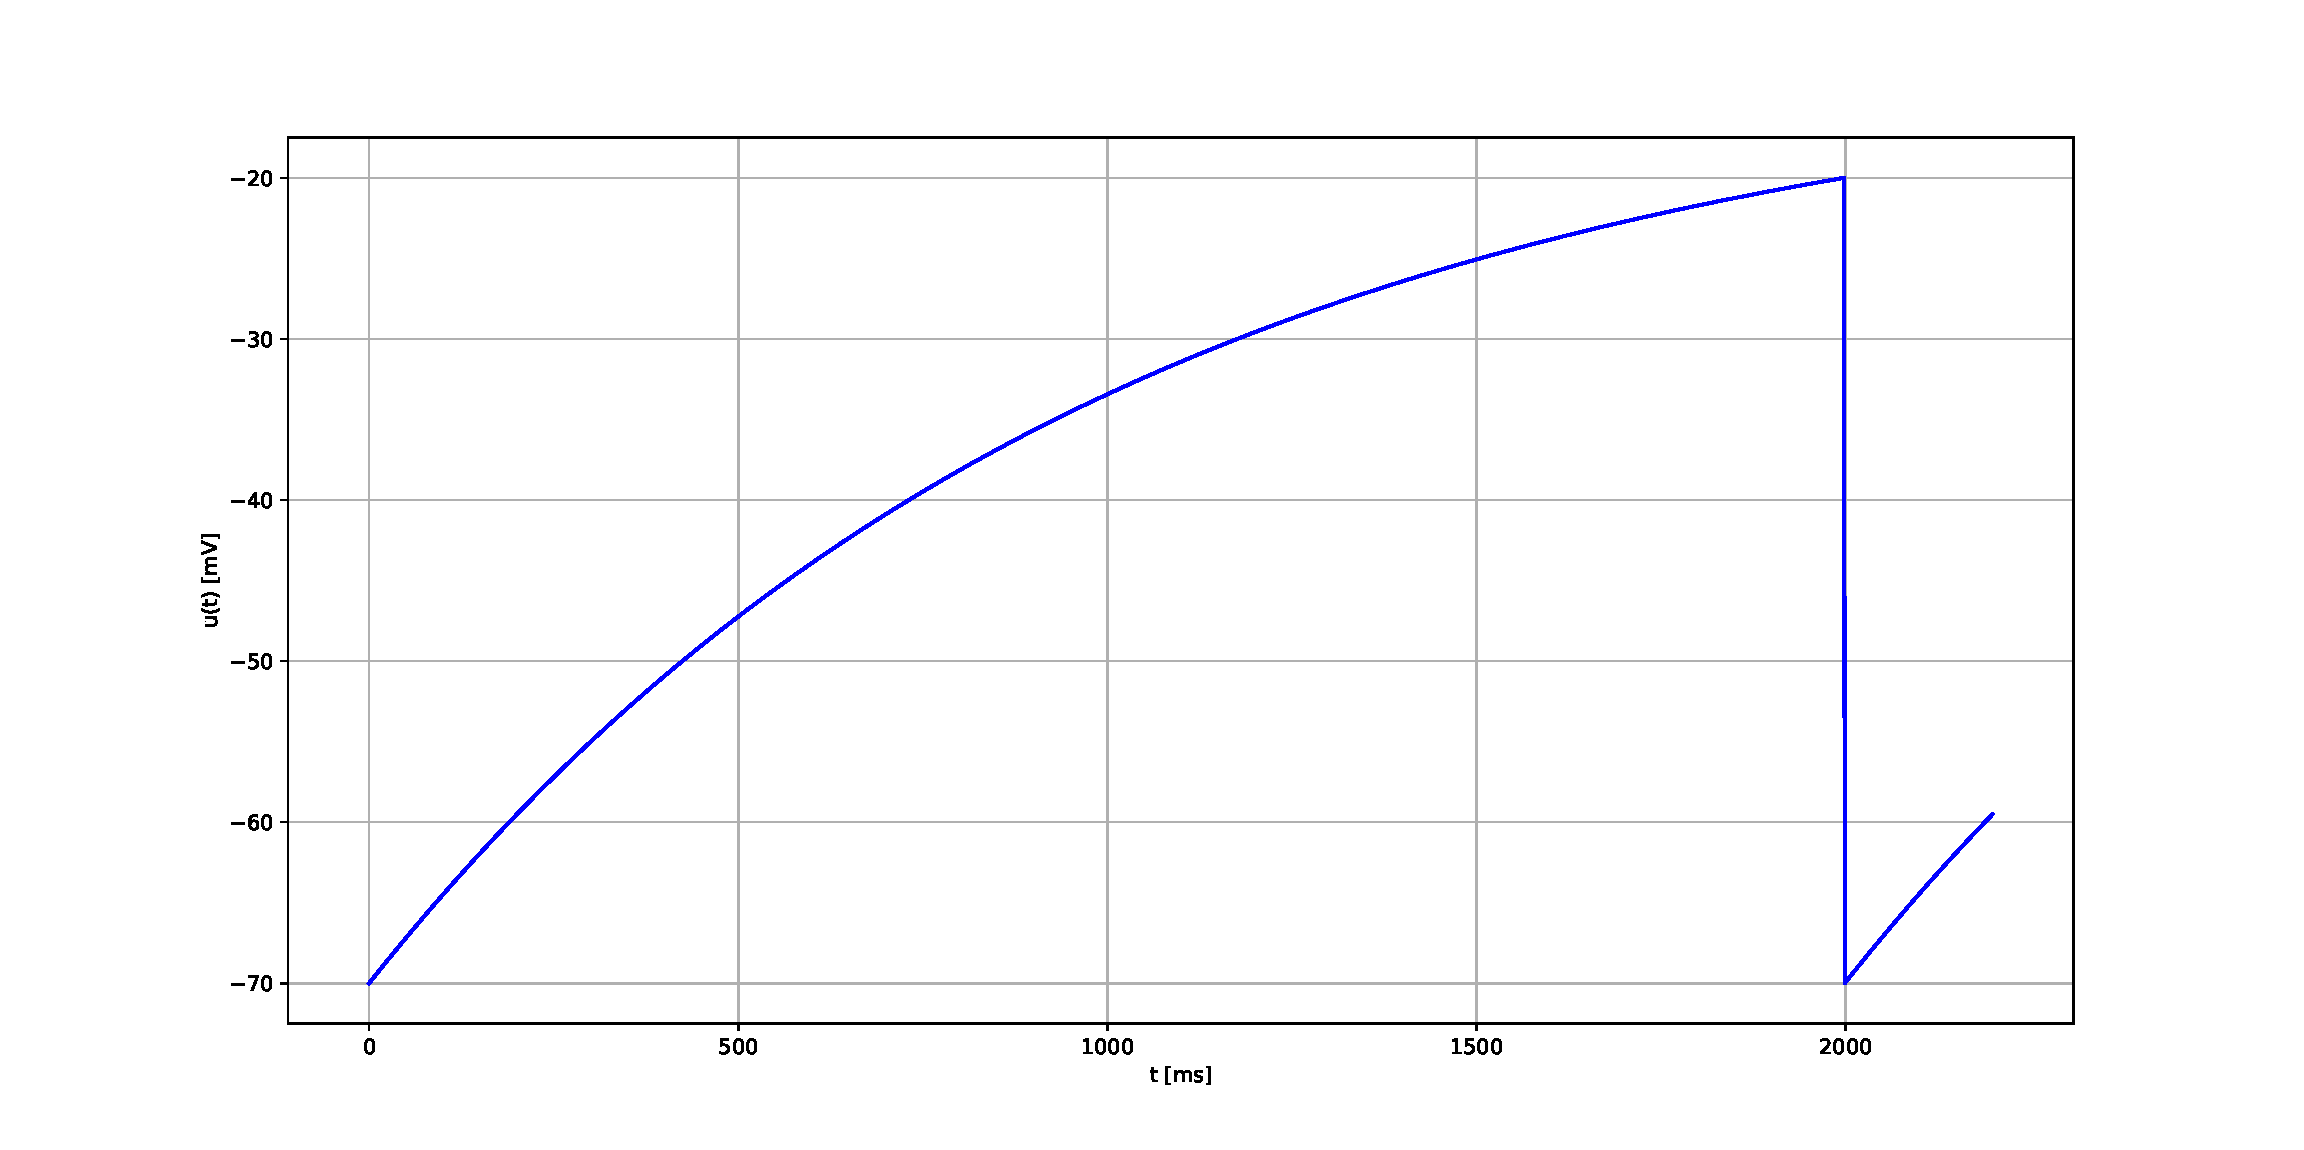
\includegraphics[width=14cm]{figures/chap_lif/Simple_LIF.pdf}
		\caption{Graphische Darstellung des Membranpotentials durch das Leaky Integrate and Fire - Modell}
		\label{fig:simple_lif}
	\end{figure}\\
	Die anliegenden Synapsenströme sind durch folgenden formularen Zusammenhang zu berechnen:
	\begin{align}
		\label{eq:chem_syn_current}
		I_{Syn} = \frac{w}{1 + \e^{\sigma(u_{pre}(t) + \mu)}}(E - u_{post}(t))
	\end{align}
	Synapsenströme sind grundsätzlich von den pre- und postsynaptischen Potentialen der jeweiligen Nervenzellen $u_{pre}$ und $u_{post}$ abhängig. Weiterhin können diese chemischen Synapsen exzitatorisch oder inhibitorisch wirken. Diese Eigenschaft wird durch das s.g. Nernstpotential $E\in[0mV, -90mV]$ beschrieben. Weitere Größen dieser Gleichung bilden $w$, die Standardabweichung $\sigma$ und $\mu$.\\
	Gap-Junctions bilden die Ausnahme, denn sie dienen als Ausgleichsglied und wirken bidirektional. Ihr Strom wird wie folgt berechnet:
	\begin{align}
		\label{eq:gap_syn_current}
		I_{Gap} = \hat{w}(u_{post}(t) - u_{pre}(t))
	\end{align}
	Für die Berechnung des Gap-Junction Stroms benötigt es ebenfalls das pre und postsynaptische Potential der jeweiligen Nervenzellen $u_{pre}$ und $u_{post}$, sowie $\hat{w}$.\\	
	Durch diese formularen Zusammenhänge kann ein ganzheitliches neuronales Netz simuliert werden.
	
% ***
\section{Anwendung auf Modelle neuronaler Netze}
\label{sec:lif_neuro}
% ***
	Durch das im vorherigen Kapitel beschriebene Leaky Integrate and Fire - Modell ist es möglich, interne Vorgänge eines neuronalen Netzes zu beschreiben und zu simulieren. Dies setzt jedoch einen konstanten Input der vier Sensorneuronen durch äußere Stimuli voraus. Diese Rezeptorneuronen sind in der Lage, äußere Einflüsse wie bspw. Licht- oder Berührungsintensität in ein für das neuronale Netz verständliche Größe zu übersetzen. Wie bereits eingangs erwähnt, bewegen wir uns in einem Aktionsraum $A\in[-70mV, -20mV]$, wobei $-70mV$ als Ruhespannung und $-20mV$ als Aktionspotential wahrgenommen wird. Aufgabe der vier Sensor-Neuronen \textit{PVD, PLM, AVM und ALM} ist es folglich, eingehende Größen entsprechend auf den gegebenen Aktionsraum $A$ zu übersetzen.\\
	In dem bereits thematisierten Schaubild nach Lechner et al (Abb. \ref{fig:01_TW-Circuit} \cite{WormLevelRL}) werden jeweils zwei Sensorneuronen für einen Eingang genutzt, da zwischen positiven und negativen Eingangsgrößen unterschieden wird. \textit{PLM und AVM} bilden das primäre Sensorpaar für die ausschlaggebendste Eingangsgröße (inverses Pendel: Winkel $\varphi$), \textit{PVD und ALM} bedienen eine sekundäre Eingangsgröße (inverses Pendel: Winkelgeschwindigkeit $\dot{\varphi}$ oder Kartposition $x$). Diese Wahl beruht auf der internen Verschaltung des Netzwerks durch Synapsen und Gap-Junctions und wird im weiteren Verlauf dieser Arbeit weiter thematisiert.\\
	Um nun die jeweiligen Größen durch die Sensorneuronen zu übersetzen werden folgende Funktionen für die jeweils positive und negative Sensorneurone $S_{positiv}$ und $S_{negativ}$ angenommen:
	\begin{align}
		\label{eq:sensor_translation_p}
		S_{positiv} &:= \begin{cases}-70mV & x\leq 0\\-70mV + \frac{50mV}{x_{min}}x & 0 < x \leq x_{min} \\-20mV & x > x_{max}  \end{cases}\\
		\label{eq:sensor_translation_n}
		S_{negativ} &:= \begin{cases}-70mV & x\geq 0\\-70mV + \frac{50mV}{x_{min}}x & 0 > x \geq x_{min} \\-20mV & x < x_{max}  \end{cases}
	\end{align}
	$x\in[x_{min}, x_{max}]$ ist eine messbare, dynamische Systemvariable, welche in den gegebenen Grenzen $x_{min} $ und $x_{max}$ auftritt. Lediglich eine Fallunterscheidung wird getroffen: nimmt $x$ einen positiven Wert an, wird Sensorneurone $S_{positiv}$ aktiviert, bei negativem $x$-Wert, agiert die Sensorneurone $S_{negativ}$.\\
	Analog lässt sich dieser Zusammenhang auf die beiden Motorneuronen \textit{REV} und \textit{FWD} übertragen. Hier werden die Signale der internen Nervenzellen \textit{AVA} und \textit{AVB} auf interpretierbare Größen in die Außenwelt übersetzt. Biologisch kann dies ein Nervenimpuls sein, welcher eine spezielle Muskelgruppe anspricht oder einen Reflex auslöst. In der hier genannten Simulationsumgebung des inversen Pendels entspricht der Ausgang des Netzwerks entweder einer diskreten Vorwärts- oder Rückwärtsbewegung. Genaueres zu der Interaktion mit dem genannten Simulationskonstrukt im Kapitel \ref{chap:imp}.

% ***
\section{Zuverlässigkeit und Limitationen}
\label{sec:lif_lim}
% ***
	Das Leaky Integrate and Fire - Modell ist stark vereinfacht und zeigt die grundsätzlichen Eigenschaften des Membranpotentials auf. Es erfolgt ein lineares Aufintegrieren der anliegenden Ströme und eine simple Rücksetzung des Aktionspotentials nach Überschreitung des Thresholds $\vartheta$ auf das Ruhepotential $U_{Leak}$.\\
	Zur weiteren Analyse eines neuronalen Netzwerks besonders im Bereich der Biologie und Biochemie werden daher detailliertere Modelle angewendet um biologische Effekte in verschiedenen Zelltypen zu berücksichtigen. Jedoch eignet sich das hier angewendete Modell sehr gut zur Analyse der gegebenen Nervenzellen. Das Leaky Integrate and Fire - Modell ist in der Lage, s.g. Fire-Events bei der Überschreitung des genannten Thresholds exakt zu ermitteln und liefert somit eine grundlegende Zeitbasis für die Simulationsumgebung.

% ***
\section{Implementierung}
\label{sec:lif_imp}
% ***
	Zur Implementierung des Leaky Integrate and Fire - Modells wird die Programmiersprache \texttt{Python} verwendet. Angelehnt an die Formeln aus \ref{sec:lif_model} kann ein einfacher Algorithmus implementiert werden. Der gesamte Code findet sich in Anhang \ref{sec:lifpy}.\\
	Da sich in der Berechnung der Membranpotentiale eine lineare Differentialgleichung erster Ordnung ergibt \ref{eq:lif}, muss diese entsprechend numerisch gelöst werden. Die Lösung kann durch das Euler-Verfahren, sowie durch die Methode nach Runge-Kutta gefunden werden, wobei letztere Methode (4. Ordnung) deutlich genauer ist.
	
	\begin{remark}[Numerisches Lösungsverfahren nach Euler]\\
		Gegeben sei eine Differentialgleichung der Form $\dot{x} = f(x)$ mit der Bedingung $x = x_0$ bei $t = t_0$. Man finde einen Weg, um die Lösung $x(t)$ zu approximieren.\\
		Weiterhin sollte die Schrittweite $\Delta t$ bekannt sein sowie die Anzahl der Zeitschritte $T$. Somit lässt sich die Differentialgleichung numerisch lösen:
		\begin{align}
			\label{eq:euler}
			x_{n+1} = x_n + f(x_n) \Delta t
		\end{align}
		Aus \cite{NonlinearDynamics}.
	\end{remark}
	\begin{remark}[Numerisches Lösungsverfahren nach erweiterter Euler-Methode]\\
		Gegeben sei ebenfalls eine Differentialgleichung der Form $\dot{x} = f(x)$ mit der Bedingung $x = x_0$ bei $t = t_0$. Man finde einen Weg, um die Lösung $x(t)$ zu approximieren.\\
		Weiterhin sollte die Schrittweite $\Delta t$ bekannt sein sowie die Anzahl der Zeitschritte $T$. Somit lässt sich die Differentialgleichung numerisch lösen:
		\begin{align}
			\label{eq:erw_euler}
			\tilde{x}_{n+1} &= x_n + f(x_n) \Delta t\\
			x_{n+1} &= x_n + \tfrac{1}{2}[f(x_n) + f(\tilde{x}_{n+1})]\Delta t
		\end{align}
		Dieses Verfahren ermöglicht eine genauere Approximation als die einfache Euler-Methode bei gleichbleibender Schrittweite. Der Fehler $E = |x(t_n)-x_n|$ wird kleiner. Aus \cite{NonlinearDynamics}.
	\end{remark}
	\begin{remark}[Numerisches Lösungsverfahren nach Runge-Kutta 4. Ordnung]\\
		Gegeben sei eine Differentialgleichung der Form $\dot{x} = f(x)$ mit der Bedingung $x = x_0$ bei $t = t_0$. Man finde einen Weg, um die Lösung $x(t)$ zu approximieren.\\
		Weiterhin sollte die Schrittweite $\Delta t$ bekannt sein sowie die Anzahl der Zeitschritte $T$. Somit lässt sich die Differentialgleichung numerisch lösen:
		\begin{align}
			\begin{split}
			\label{eq:runkgekutta}
			k_1 &= f(x_n) \Delta t\\
			k_2 &= f(x_n + \tfrac{1}{2} k_1) \Delta t\\
			k_3 &= f(x_n + \tfrac{1}{2} k_2) \Delta t\\
			k_4 &= f(x_n + k_3) \Delta t\\
			\end{split}\\[10pt]
			x_{n+1} &= x_n + \tfrac{1}{6} (k_1 + 2 k_2 + 2 k_3 + k_4)
		\end{align}
		Dieses Verfahren ermöglicht eine genauere Approximation als die Euler-Methoden bei gleichbleibender Schrittweite. Der Fehler $E = |x(t_n)-x_n|$ wird signifikant kleiner. Diese Methode erfordert jedoch eine höhere Rechenzeit und ist daher nur bei ausreichender Leistung anzuwenden. Aus \cite{NonlinearDynamics}.
	\end{remark}
	Anwendung der Anmerkung 2.3 auf die Funktion \ref{eq:lif} resultiert in folgende Berechnung, welche direkt implementiert werden kann:
	\begin{equation}
	\begin{split}
		\label{eq:runkgekutta_nn}
		k_1 &= \frac{(G_{leak} (U_{leak} - u_i(t)) + (I_{Stimuli} + I_{Syn} + I_{Gap}))}{C_m} \Delta t\\
		k_2 &= \frac{(G_{leak} (U_{leak} - (u_i(t) + \tfrac{1}{2} k_1)) + (I_{Stimuli} + I_{Syn} + I_{Gap}))}{C_m} \Delta t\\
		k_3 &= \frac{(G_{leak} (U_{leak} - (u_i(t) + \tfrac{1}{2} k_2)) + (I_{Stimuli} + I_{Syn} + I_{Gap}))}{C_m} \Delta t\\
		k_4 &= \frac{(G_{leak} (U_{leak} - (u_i(t) + k_3)) + (I_{Stimuli} + I_{Syn} + I_{Gap}))}{C_m} \Delta t
	\end{split}
	\end{equation}
	Rekursive Berechnung der vier Koeffizienten führt zum neuen Membranpotential und entsprechend zu der Information, ob die internen Nervenzellen \textit{AVA} oder \textit{AVB} gefeuert haben:
	\begin{align}
		\label{eq:runkgekutta_erg}
		u_{i+1}(t) &= u_i(t) + \tfrac{1}{6} (k_1 + 2 k_2 + 2 k_3 + k_4)
	\end{align}
	Um diese Funktion im Gesamtcode später mühelos aufrufen zu können, wird ein Python-Script (\texttt{modules/lif.py}) erstellt. Dieses enthält neben der Funktion zur Berechnung des Membranpotentials auch die der Berechnung von Synapsen- und Gap-Junction-Strömen. Das gesamte Modul zur Berechnung von Strömen und Spannungen pro Zeiteinheit wird wie folgt implementiert:
	\begin{algorithm}
		\SetKwInOut{Input}{Input}
		\SetKwInOut{Output}{Output}
		
		\Input{$\boldsymbol{x}, \boldsymbol{u}, \boldsymbol{A}, \boldsymbol{B}, \boldsymbol{C_m}, \boldsymbol{G_{Leak}}, \boldsymbol{U_{Leak}}, \boldsymbol{\sigma}, \boldsymbol{w}, \boldsymbol{\hat{w}}$}
		\Output{Simulationsinformation (information.txt), Parameter-Dump als .hkl Datei}
		
		\For{i $\leftarrow$ 1 \textbf{to} 4}{
			\For{j $\leftarrow$ 1 \textbf{to} 4}{
				$I_inter{i,j}$ = I\_syn\_calc($x[i], x[j], E, w[k], \sigma[k], \mu$)\\
				$I_sensor{i,j}$ = I\_syn\_calc($u[i], u[j], E, w[k], \sigma[k], \mu$)\\
				k $\leftarrow$ k + 1
				$I_gap{i,j}$ = I\_gap\_calc($x[i], x[j], \hat{w[k]}$)\\
			}
		}
		\KwRet{information.txt, parameter\_dump.hkl, date, best\_reward}
		\caption{compute}
	\end{algorithm}

%%% Local Variables: 
%%% mode: latex
%%% TeX-master: "main"
%%% End: 
